%%%%%%%%%%%%%%%%%%%%%%%%%%%%%%%%%%%%%%%%%%%%%%%%%%%%%%%%%%%%%%%%%%%%%%%%%%%%%%%%
\chapter{Placement Algorithms}
\label{ch:placement}
%%%%%%%%%%%%%%%%%%%%%%%%%%%%%%%%%%%%%%%%%%%%%%%%%%%%%%%%%%%%%%%%%%%%%%%%%%%%%%%%

The input for a placement algorithm consists of the deposition sequence $N$,
a set of probes $\mathcal{P}$ (each probe is assumed to have at least one
embedding in $N$) and a geometry of spots $\mathcal{S}$.

The output of a placement algorithm is a one-to-one assignment of probes to
spots. If there are more spots than probes to place, we can add enough ``empty''
probes that do not introduce any conflicts with the other probes (since light
is never directed to such spots).

All algorithms discussed in this section assume that an initial embedding
of the probes is given, which can be a left-most, right-most, synchronous or
otherwise pre-computed embedding --- a placement algorithm typically does not
change the given embeddings.


\section{Early approaches}
\label{sec:placement_early}

\begin{figure}
\begin{picture}(330,100)
\put(0,0){\makebox(110,15){a)}}
\put(110,0){\makebox(110,15){b)}}
\put(220,0){\makebox(110,15){c)}}
\put(-3,15){  \makebox(110,85){\includegraphics[width=0.3\textwidth]{0threading}}}
\put(110,15){\makebox(110,85){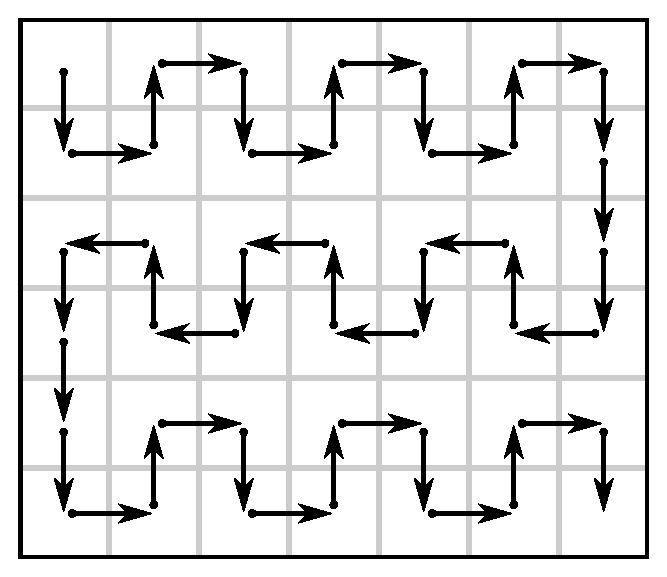
\includegraphics[width=0.3\textwidth]{1threading}}}
\put(220,15){\makebox(110,85){\includegraphics[width=0.3\textwidth]{2threading}}}
\end{picture}
\caption{\label{fig:threading}%
  Different ways of \emph{threading} probes on a chip. a) Standard
  row-by-row (0-threading); b) 1-threading; c) 2-threading.}%
\end{figure}

\citet{Feldman1994} were the first to formally address the unintended
illumination problem. They showed how an optimal placement can be constructed
based on a two-dimensional Gray code.  Their work, however, is restricted to
\emph{uniform arrays} (arrays containing all $4^\ell$ probes of a given length
$\ell$) and synchronous embeddings, being thus of limited practical importance
for current microarrays.

The border length problem on arrays of arbitrary probes was first
discussed by \citet{Hannenhalli2002}. The article reports that the
first Affymetrix chips were designed using a heuristic for the
traveling salesman problem (TSP). The idea is to build a weighted
graph with nodes representing probes, and edges containing the Hamming
distances between their embeddings, that is, the number of times their
embeddings differ at a particular synthesis step. A TSP tour on this
graph is heuristically constructed, resulting in consecutive probes in
the tour being likely similar. The TSP tour is then \emph{threaded} on
the array in a row-by-row fashion (Fig.~\ref{fig:threading}a).

Hannenhalli and co-workers studied several threading alternatives,
which they collectively called \emph{$k$-threading}
(Fig.~\ref{fig:threading}b,c). A $k$-threading is a variation of the
standard row-by-row threading, in which the right-to-left and
left-to-right paths are interspaced with alternating upward and
downward movements over $k$ sites. (The row-by-row threading can be
seen as a $k$-threading with $k=0$.) Hannenhalli and co-workers
experimentally observed that 1-threading may reduce border length in up to
20\% for large chips when compared to row-by-row threading.

A different strategy, called Epitaxial placement, was proposed by
\citet{Kahng2002}. It was originally designed for chips with synchronous
embeddings, but it can be trivially implemented for asynchronous embeddings as
well. The algorithm starts by placing a random probe in the center of the array
and continues to insert probes in spots adjacent to already-filled spots.
Priority is given to spots whose all four neighbors are full, in which case a
probe with the minimum number of border conflicts with the neighbors is placed.
Otherwise, all spots~$s$ with $i \geq 1$ filled neighbors are examined. For each
spot, the algorithm finds a non-assigned probe~$p$ whose number of conflicts
with the filled neighbors, $c(s,p)$, is minimal, and assigns a cost
$C(s,p) = k_i \cdot c(s,p) / i$ for this assignment, where $0 < k_i \leq 1$ are
scaling coefficients (the authors propose $k_1 = 1$, $k_2 = 0.8$, and
$k_3 = 0.6$). The assignment with minimum $C(s,p)$ is made and the procedure is
repeated until all probes have been placed. With this algorithm, Kahng and
co-workers claim a further 10\% reduction in border conflicts over
TSP\,+\,1-threading.

Both the Epitaxial algorithm and the TSP approach have at least quadratic time
complexity and hence do not scale well to large chips. This observation
motivated the design of two new placement algorithms: Sliding-Window Matching
(SWM) and Row-Epitaxial \citep{Kahng2003}.



\section{Sliding-Window Matching}
\label{sec:placement_swm}

\begin{figure}[t!]
\centerline{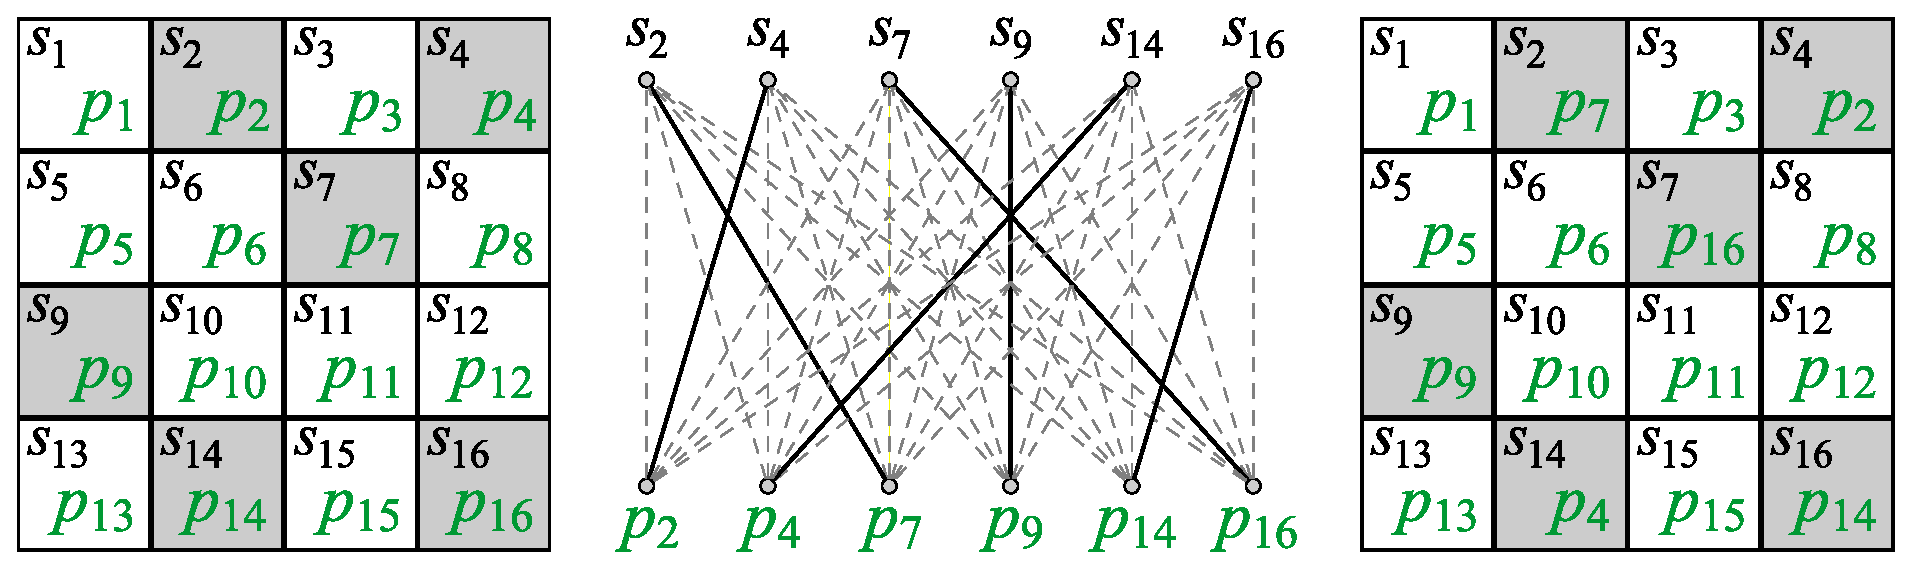
\includegraphics[width=\textwidth]{swm.eps}}
\begin{picture}(340,15)
\put(0,0){\makebox(95,15){a)}}
\put(95,0){\makebox(145,15){b)}}
\put(240,0){\makebox(95,15){c)}}
\end{picture}
\caption{\label{fig:swm}%
  Sliding-Window Matching algorithm. a) Initial arrangement of probes
  $p_1 \dots p_{16}$ inside a $4 \times 4$ window and the selected independent
  set of spots (shaded). b) Bipartite graph and a minimum weight perfect
  matching (dark edges). c) New arrangement inside the window.}%
\end{figure}

The SWM is not exactly a placement algorithm as it iteratively improves an
existing placement that can be constructed, for instance, by
TSP\,+\,1-threading, or much simpler, by lexicographically sorting the binary
embedding vectors with a linear-time radix sort. The sorting is several times
faster but it is also likely to produce a worse initial placement than the
TSP, with consecutive embeddings being similar only in their first synthesis
steps. This, however, should be of little importance given that this placement
is only used as a starting point for the SWM algorithm.

The SWM works inside a window that starts at the top left of the chip
and slides from left to right, top to bottom, while maintaining a
certain amount of overlap between each iteration. When the window
reaches the right-end of the chip, it is re-started at the left-end of
the next set of rows, also retaining an overlap with the preceding
rows.

At each iteration, the algorithm attempts to reduce the total border
length inside the window by relocating some probes
(Fig.~\ref{fig:swm}a).  First, a random maximal independent set
of spots is selected, and the probes assigned to these spots are
removed. The term independent refers to the fact that selected spots
can be re-assigned to probes without affecting the border length of
other selected spots. The algorithm creates a bipartite graph with
nodes representing the removed probes and the now vacant spots
(Fig.~\ref{fig:swm}b). The edges of this graph are weighted
with the number of border conflicts that are generated by the
corresponding assignment.  Finally, a minimum weight perfect matching
on this graph is computed, and the indicated assignments are made
(Fig.~\ref{fig:swm}c).

Selecting an independent set of spots ensures that the cost of each
new assignment can be computed independently of the other assignments.
The SWM was designed for border length minimization and it takes
advantage of the fact that, in this model, an independent set of spots
can be constructed by selecting sites that are not immediate
neighbors (spots that do not share a common border).
SWM can be adapted for conflict index minimization (to our knowledge,
this has not been implemented) by using larger windows containing
relatively sparse independent sets. Therefore several random
independent sets should be constructed before moving the window.


\section{Row-Epitaxial}
\label{sec:placement_reptx}

The Row-Epitaxial algorithm is a variant of the Epitaxial algorithm
with two main differences introduced to improve scalability: i) spots
are filled in a pre-defined order, namely, from top to bottom, left to
right, and ii) only a limited number $Q$ of probes are considered
for filling each spot.

Like SWM, Row-Epitaxial improves an initial placement that is
constructed by TSP\,+\,1-threading or Radix-sort\,+\,1-threading. For
each spot $s$ of the chip, it looks at the next $Q$ probes that lie in
close proximity (to the right or below $s$), and swaps the current
probe of $s$ with the probe that generates the minimum number of
border conflicts with the top and left neighbors of $s$.
Row-Epitaxial can be adapted to conflict index minimization by
restricting the computation of the conflict index of $s$ to those
neighboring probes that are to the left or above $s$ (those which have
already found their final positions).

Fig.~\ref{fig:rowepitaxial} shows computational results for normalized border
length and average conflict index for various chip dimensions and different
values of $Q$.  The running time of Row-Epitaxial is $O(Qn)$, i.e., linear in
the chip size, where $Q$ is a user-defined constant.  In this way, solution
quality can be traded for running time: More candidates yield better layouts
but also demand more time.  For border length minimization, increasing $Q$
above 10\,000 has little positive effect.

According to experiments conducted by \citet{Kahng2003},
Row-Epitaxial is the best known large-scale placement algorithm,
achieving up to 9\% reduction in border length over the
TSP\,+\,1-threading, whereas SWM achieves slightly worse results but
requires significantly less time.


\begin{figure}
%%
\begin{picture}(334,145)\footnotesize{
  \put(0,0){\makebox(167,145){
    %GNUPLOT: LaTeX picture with Postscript
    \begin{picture}(0,0)%
    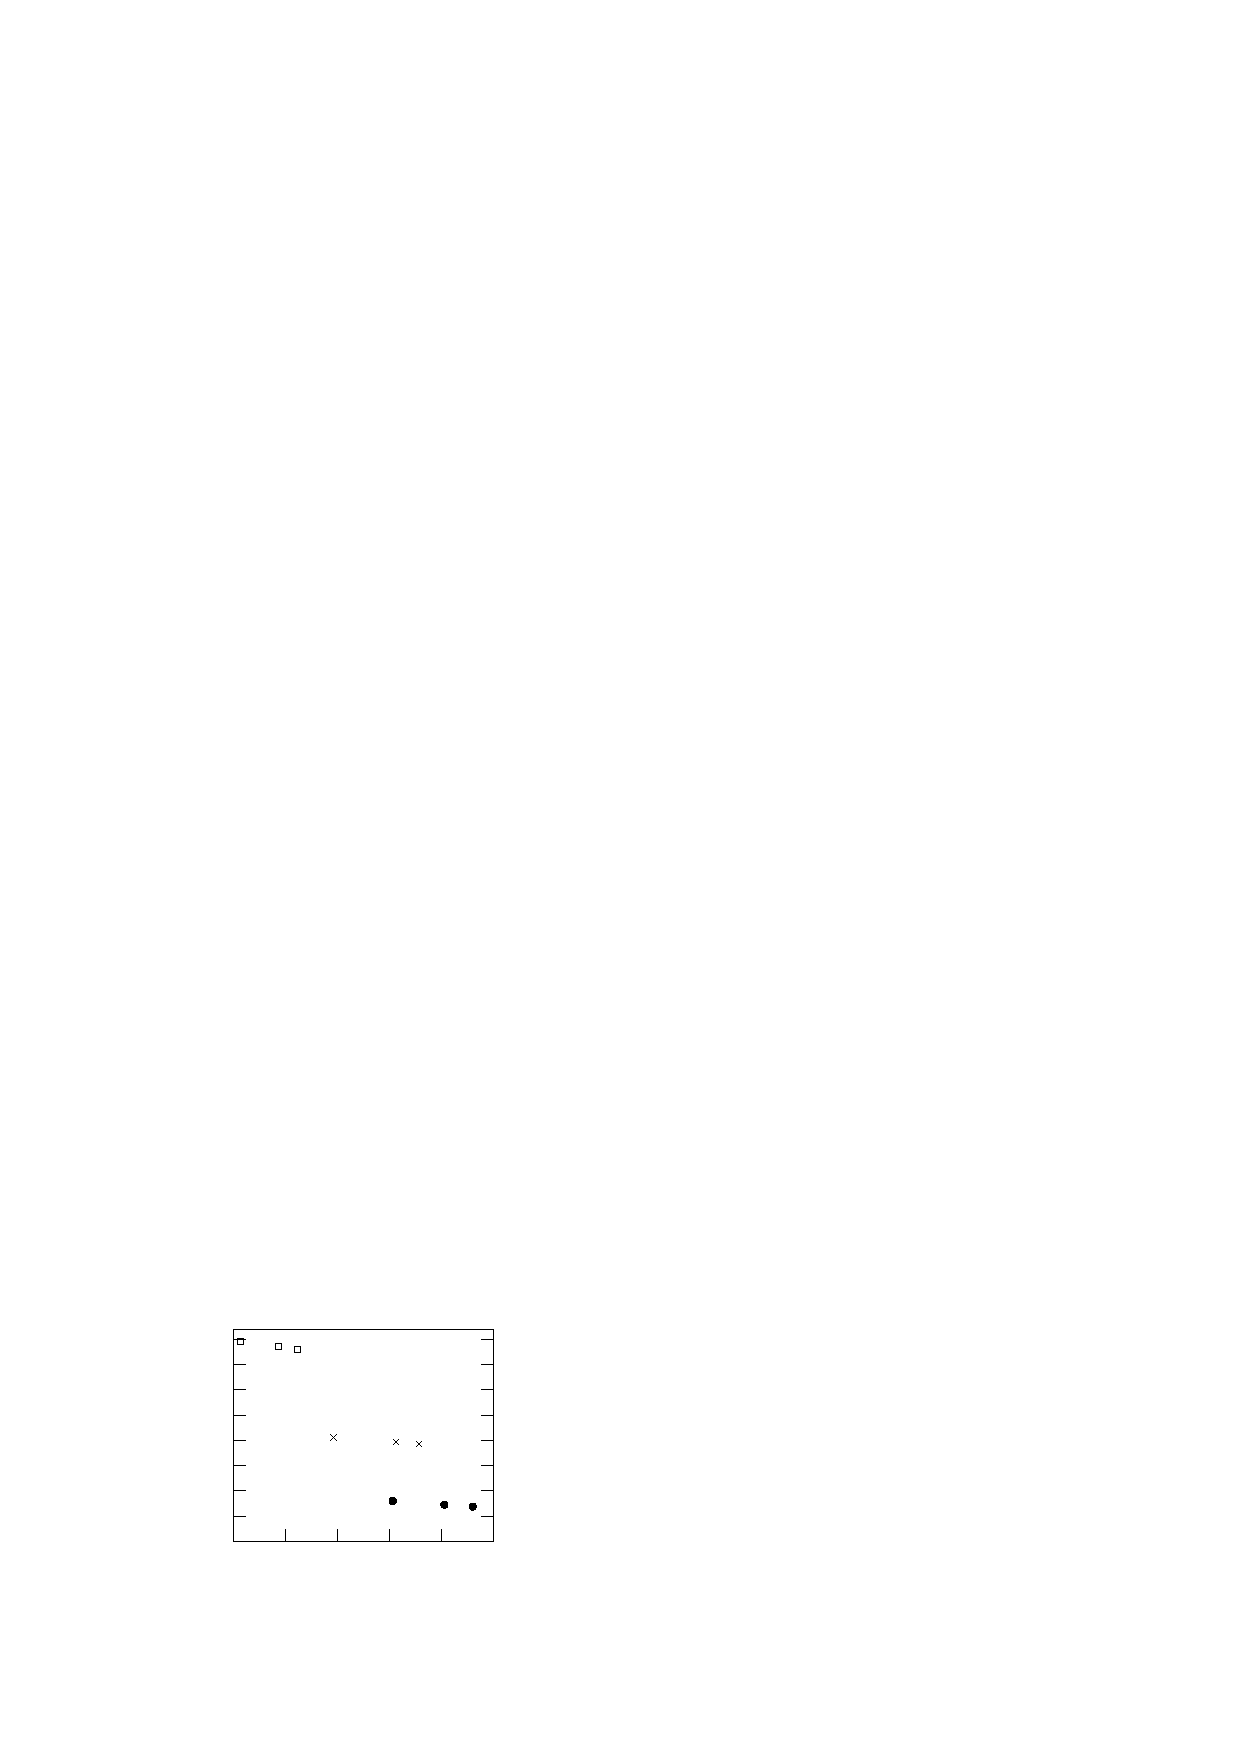
\includegraphics{reptx/reptx-bl}%
    \end{picture}%
    \begingroup
    \setlength{\unitlength}{0.0200bp}%
    \begin{picture}(9000,8100)(0,0)%
    \put(1750,1500){\makebox(0,0)[r]{\strut{} 44}}%
    \put(1750,2107){\makebox(0,0)[r]{\strut{} 44.5}}%
    \put(1750,2714){\makebox(0,0)[r]{\strut{} 45}}%
    \put(1750,3321){\makebox(0,0)[r]{\strut{} 45.5}}%
    \put(1750,3929){\makebox(0,0)[r]{\strut{} 46}}%
    \put(1750,4536){\makebox(0,0)[r]{\strut{} 46.5}}%
    \put(1750,5143){\makebox(0,0)[r]{\strut{} 47}}%
    \put(1750,5750){\makebox(0,0)[r]{\strut{} 47.5}}%
    \put(1750,6357){\makebox(0,0)[r]{\strut{} 48}}%
    \put(2000,1000){\makebox(0,0){\strut{} 8}}%
    \put(3250,1000){\makebox(0,0){\strut{} 16}}%
    \put(4500,1000){\makebox(0,0){\strut{} 32}}%
    \put(5750,1000){\makebox(0,0){\strut{} 64}}%
    \put(7000,1000){\makebox(0,0){\strut{} 128}}%
    \put(8250,1000){\makebox(0,0){\strut{} 256}}%
    \put(5125,250){\makebox(0,0){\strut{}Time (min)}}%
    \put(5125,7350){\makebox(0,0){\strut{}Normalized border length}}%
    \end{picture}%
    \endgroup
  }}
  \put(167,0){\makebox(167,145){
    %GNUPLOT: LaTeX picture with Postscript
    \begin{picture}(0,0)%
    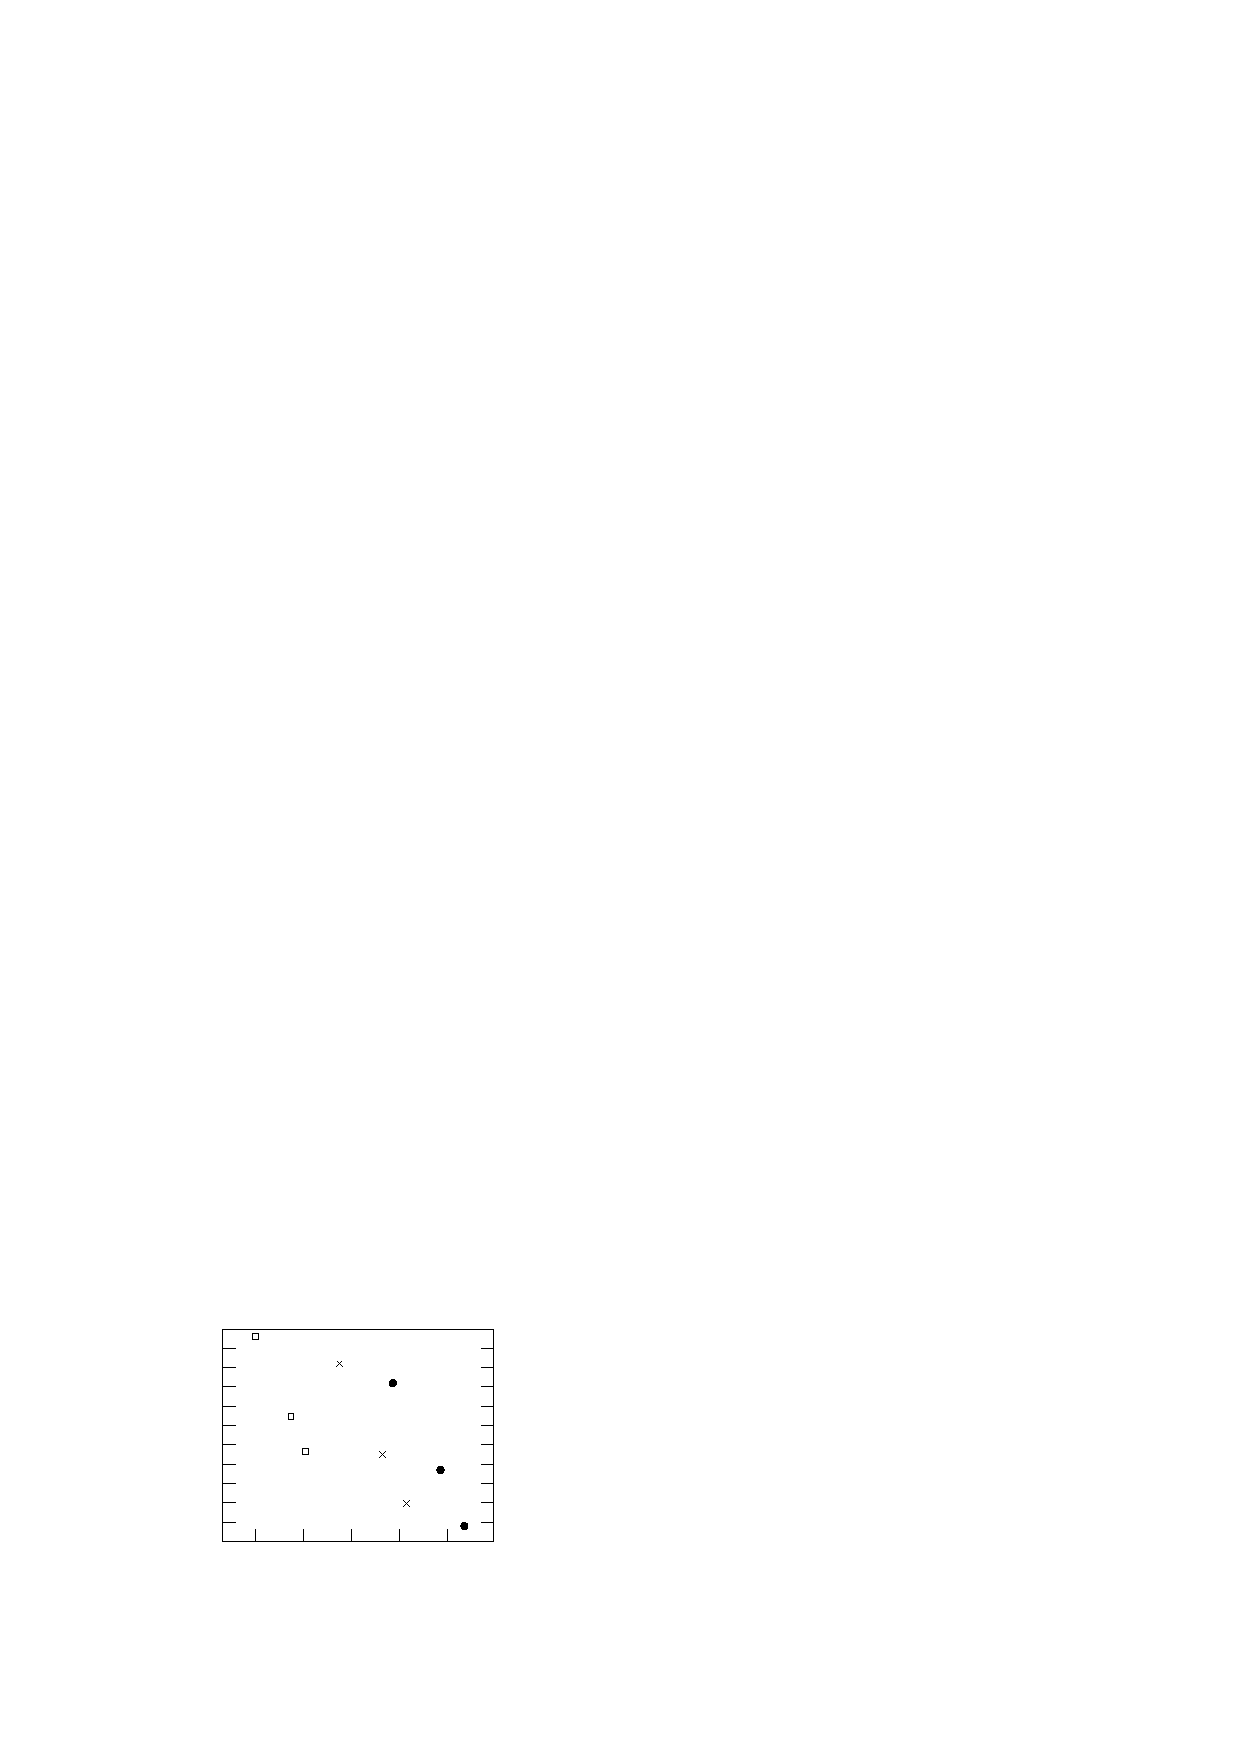
\includegraphics{reptx/reptx-ci}%
    \end{picture}%
    \begingroup
    \setlength{\unitlength}{0.0200bp}%
    \begin{picture}(9000,8100)(0,0)%
    \put(1500,1500){\makebox(0,0)[r]{\strut{} 535}}%
    \put(1500,1964){\makebox(0,0)[r]{\strut{} 540}}%
    \put(1500,2427){\makebox(0,0)[r]{\strut{} 545}}%
    \put(1500,2891){\makebox(0,0)[r]{\strut{} 550}}%
    \put(1500,3355){\makebox(0,0)[r]{\strut{} 555}}%
    \put(1500,3818){\makebox(0,0)[r]{\strut{} 560}}%
    \put(1500,4282){\makebox(0,0)[r]{\strut{} 565}}%
    \put(1500,4745){\makebox(0,0)[r]{\strut{} 570}}%
    \put(1500,5209){\makebox(0,0)[r]{\strut{} 575}}%
    \put(1500,5673){\makebox(0,0)[r]{\strut{} 580}}%
    \put(1500,6136){\makebox(0,0)[r]{\strut{} 585}}%
    \put(1500,6600){\makebox(0,0)[r]{\strut{} 590}}%
    \put(2531,1000){\makebox(0,0){\strut{} 16}}%
    \put(3683,1000){\makebox(0,0){\strut{} 32}}%
    \put(4834,1000){\makebox(0,0){\strut{} 64}}%
    \put(5986,1000){\makebox(0,0){\strut{} 128}}%
    \put(7138,1000){\makebox(0,0){\strut{} 256}}%
    \put(5000,250){\makebox(0,0){\strut{}Time (min)}}%
    \put(5000,7350){\makebox(0,0){\strut{}Average conflict index}}%
    \end{picture}%
    \endgroup
  }}
}\end{picture}
%%
\caption{\label{fig:rowepitaxial}
  Trade-off between solution quality and running time with the
  Row-Epitaxial algorithm, on random chips of dimensions $200 \times
  200$ ({\tiny $\Box$}), $300 \times 300$ ({\tiny $\times$}) and $500
  \times 500$ ({\tiny $\bullet$}).  The number $Q$ of candidates per
  spot are $10\,000$, $20\,000$, and $30\,000$ from left to right.
  Layouts are measured by normalized border length (left) and average
  conflict index (right).}
\end{figure}
